\documentclass[a4paper]{scrartcl}
\usepackage[dvipsnames]{xcolor}
\usepackage[english]{babel}
\usepackage[utf8]{inputenc}
\usepackage{booktabs}
\usepackage{float}
\usepackage{hyperref} 
\usepackage{graphicx}
\usepackage{listings}
\usepackage[style=ieee]{biblatex}
\usepackage{subcaption}
\usepackage{todonotes}
\usepackage{fancyvrb}

\addbibresource{bibliography.bib}

\renewbibmacro*{bbx:savehash}{}

\RecustomVerbatimCommand{\VerbatimInput}{VerbatimInput}%
{fontsize=\footnotesize,
 %
 frame=lines,  % top and bottom rule only
 framesep=2em, % separation between frame and text
 rulecolor=\color{Gray},
 %
 label=\fbox{\color{Black}LICENSE},
 labelposition=topline,
 %
 commandchars=\|\(\), % escape character and argument delimiters for
                      % commands within the verbatim
 commentchar=*        % comment character
}
%----------------------------------------------------------------------------------------
%	TITLE SECTION
%----------------------------------------------------------------------------------------
\title{Traffic-dependent routing based on OpenStreetMap data and TMC messages}

\author{
  Jan Strauß\\
  Matr.-Nr. 2727381\\
  swt85730@stud.uni-stuttgart.de
}

\date{}
%----------------------------------------------------------------------------------------
\begin{document}
\maketitle

\abstract{
In this report a routing application that uses data from the OpenStreetMap project and Traffic Message Channel (TMC) messages to provide traffic-dependent routing on a web-based user interface is presented. This application was developed within the context of the \textit{Fachpraktikum: Algorithms for OpenStreetMap data} course during the summer semester 2016 at the University of Stuttgart.}

%----------------------------------------------------------------------------------------
%	ARTICLE CONTENTS
%----------------------------------------------------------------------------------------
\section{Introduction}
Participants of the course \textit{Fachpraktikum: Algorithms for OpenStreetMap data} were tasked to build a routing application that uses OpenStreetMap \cite{osm_main} data to provide distance and time based routing for cars, bikes and pedestrians. After this base task was completed, the routing application should be extended. This application was extended to use current traffic information as available via the TMC radio broadcasts for the route calculation, e.g. route around a traffic congestion. The result is depicted in Figure \ref{fig:tmc_comp}. A similar system was realized by \citeauthor{sanwald2013} in the context of a bachelor thesis \cite{sanwald2013}. While the implementation by \citeauthor{sanwald2013} is Java-based, the application presented in this report is written in Rust \cite{rust_main}. Rust is a new system programming language with strong guarantees on memory and thread safety. The language fits the requirements for a routing application very well: It is a compiled language that offers performance on-par with C++, the standard library contains easy to work with collection types and the language ecosystem offers libraries that provide needed features like a Http server or a parser for pbf files (the OpenStreetMap data format). For a more in-depth discussion see section \ref{impl}.

\begin{figure}
    \centering
    \begin{subfigure}[b]{0.4\textwidth}
        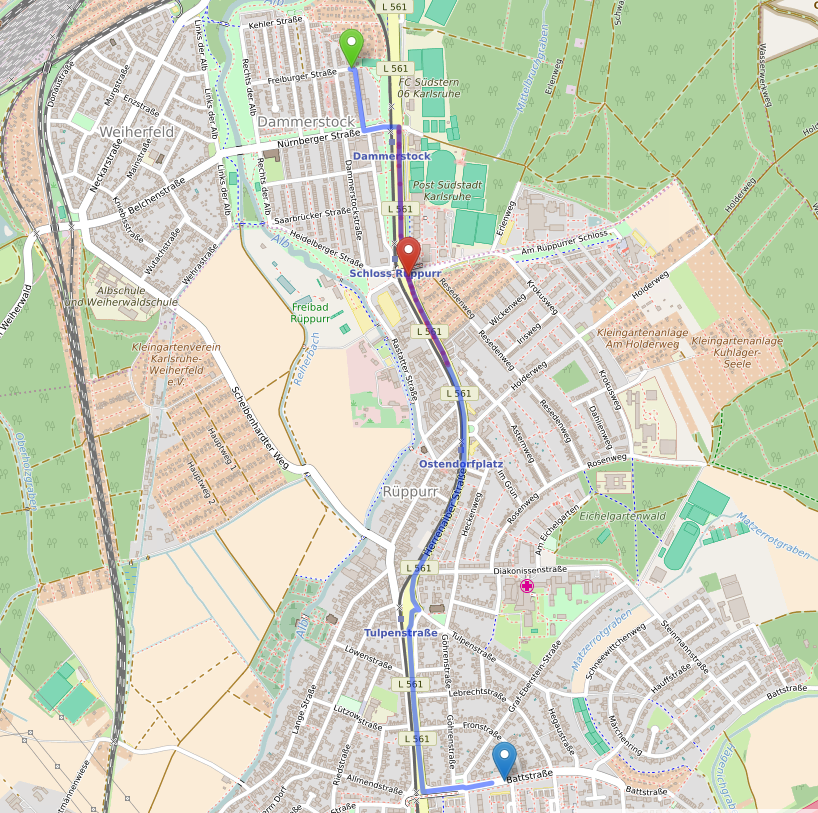
\includegraphics[width=\textwidth]{img/no_tmc.png}
        \caption{Ignoring TMC Events in the route calculation.}
        \label{fig:no_tmc}
    \end{subfigure}
    ~ %add desired spacing between images, e. g. ~, \quad, \qquad, \hfill etc. 
      %(or a blank line to force the subfigure onto a new line)
    \begin{subfigure}[b]{0.4\textwidth}
        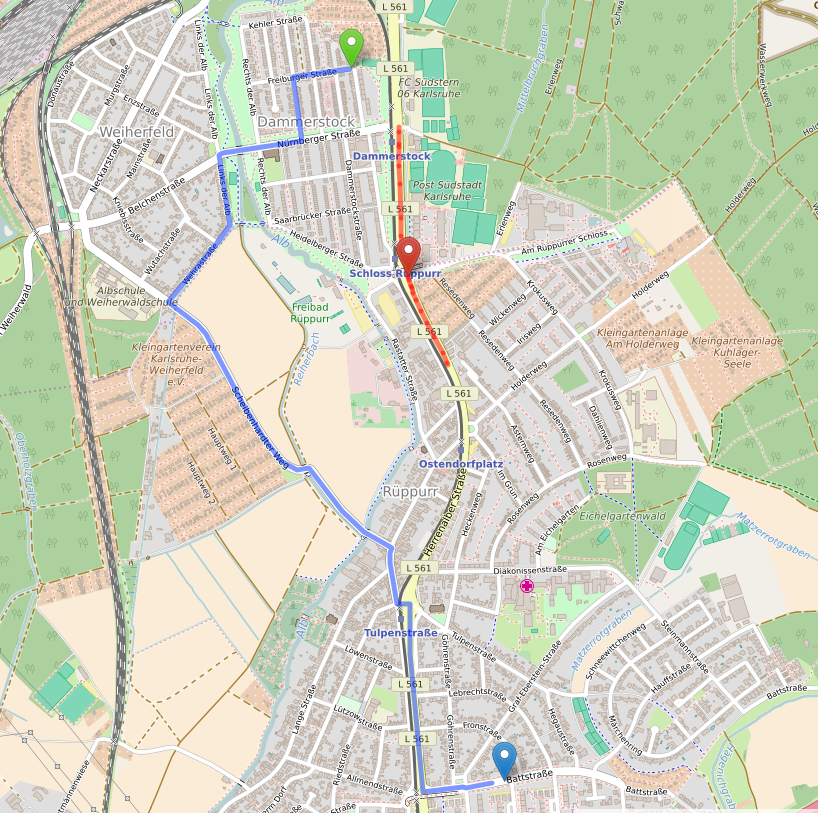
\includegraphics[width=\textwidth]{img/with_tmc.png}
        \caption{Respecting TMC Events in the route calculation.}
        \label{fig:with_tmc}
    \end{subfigure}
    \caption{Effect of respecting TMC events in the route calculation on the shortest found route for the same start and end points.}\label{fig:tmc_comp}
\end{figure}

The remainder of this report is structured as followed: First, the OpenStreetMap data format and TMC concepts are presented in section \ref{bg}. In the next section, \ref{sys}, the system is presented and in section \ref{impl} some implementation details are presented. Finally a conclusion and possible future work is presented in section \ref{concl}.

\section{Background}
\label{bg}
\subsection{OpenStreetMap (OSM)}
OpenStreetMap \cite{osm_main} is a project that aims to build a free map of the world. The geographical information is contributed by over 3 million users worldwide and the database contains over 3.5 billion nodes and over 370 million ways \cite{osm_stats}, the primitive data types the map is build from. The data can be freely downloaded and used and there are extracts available that are limited to certain areas (e.g. country, continent, region, city). The data can be downloaded in different formats, where to most efficient one is the *.osm.pbf binary format, that is also used by this application. The primitive data types have their associated information stored in key-value pairs called tags. For more information about the *.osm.pbf format and the data types used by OSM, see section \ref{sec:parsing}

\subsection{Traffic Message Channel (TMC)}
The Traffic Message Channel is a service that broadcasts traffic information. It is typically received via RDS, the Radio Data System, a standard to embed digital information in FM radio transmissions. TMC messages consist of a location code, an event code, the direction, incident extend and other fields that we will ignore here. The location code is defined in a document called LCL, the location code list. A location can have a neighbor location in positive and negative direction and the extend field of a TMC message is measured in hops over neighbors in the direction of the direction field of the message. The event codes are defined in the ECL, the event code list. So with the information from TMC messages one can determine the type of event, the location, direction and extend using the LCL and ECL. To use TMC messages in combination with routing based on OSM data two problems have to be solved: First it is necessary to have a mapping from TMC location code to the corresponding OSM data entry. Luckily the OSM dataset contains TMC Tags for some of its ways. The second problem is to determine the slowdown of a event code. To solve this, a simple lookup table is build, see section \ref{sec:tmc_handling}. 

For Germany, a new tagging scheme for TMC-data was proposed and is widely adopted today. This new scheme drastically simplifies the handling of TMC tags. The new tagging format uses the string "tmc" as key and a string in the form of "DE:1234+5678". The first number is the current location id, the + is used to describe the postive direction and the second number describes the next location id in the posiive direction. There are, respectively, the - sign for the negative direction and the / sign, which is a shorthand for A+B and B-A. More information about the new scheme can be found at \cite{osm_wiki_tmc_new_scheme}.

\section{System}
\label{sys}
The general architecture of the system is shown in Figure \ref{arch}. A OSM extract in the pbf format is used as input by the parser to build the routing graph and to generate other routing information (see section \ref{data_representation}). This state can be saved to disk and be loaded upon start, so that not every restart of the system causes the parser to run. The State is used by the Routing module which is called by the HTTP-Server when a routing request was received from the web-UI. The HTTP-Server also serves the static content of the web-UI, e.g. the leaflet library. The TMC module starts the RDSD and RDSQUERY binaries and reads the STDOUT of RDSQUERY and generates new TMC events from this data source and updates the State appropriately.

\begin{figure}[t]
\centering
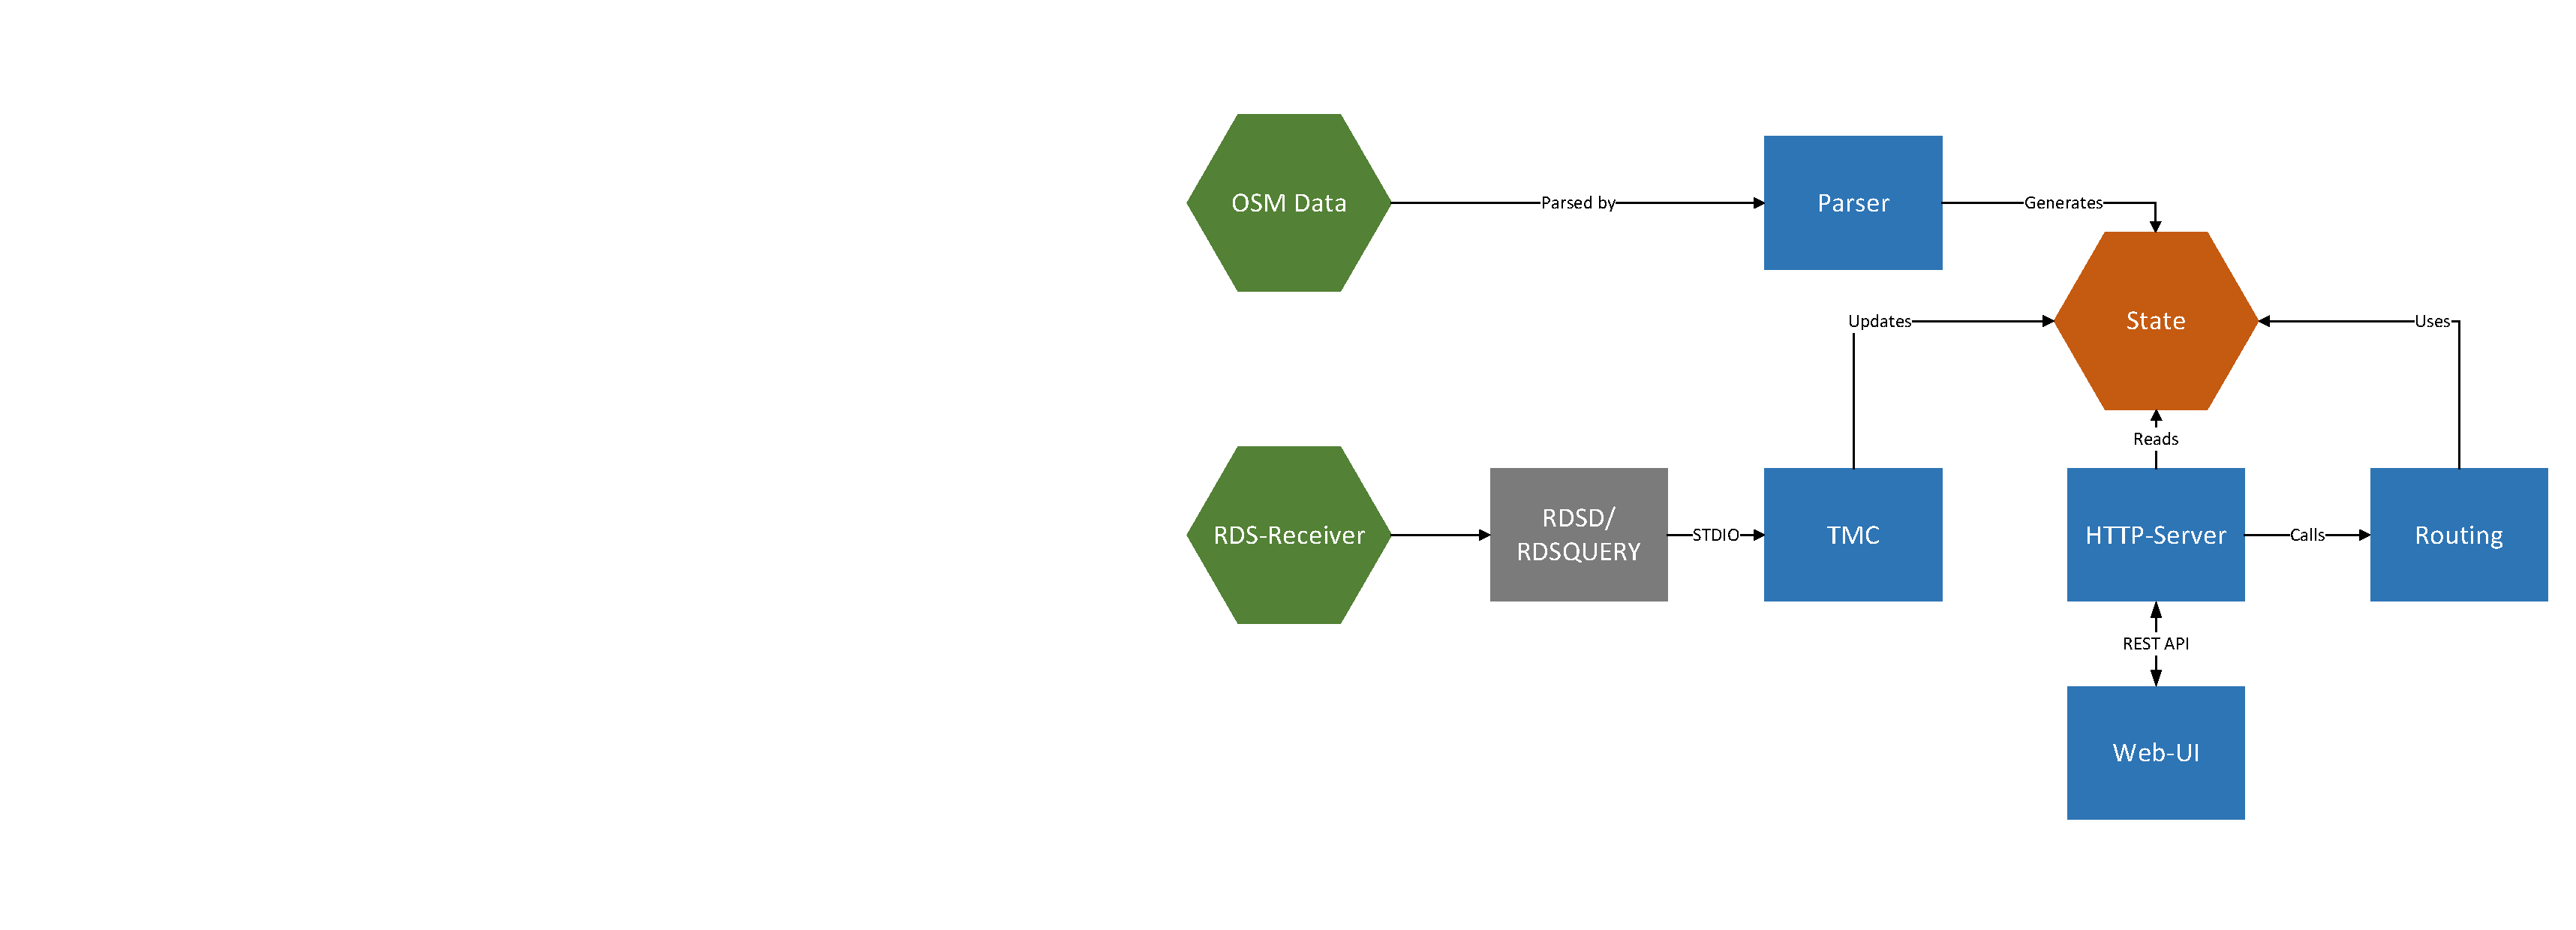
\includegraphics[width=1.0\textwidth]{img/arch_overview.pdf}
\caption{Architectural overview. Modules are blue, input artifacts green and the internal state orange.}
\label{arch}
\end{figure}

\subsection{Parsing OSM data}
\label{sec:parsing}
OpenStreetMap provides its map data in different formats, e.g. PBF or XML. The PBF (Protocolbuffer Binary Format) is the most efficient format. It is based on Googles Protobuf library. The File format uses serveral tricks to reduce the file size which makes reading such files complicated. However several libraries provide conviniernt wrappers that read the files and offer a abstraction similar to the general data primitives OSM offers. 

These primitives are Nodes, Ways and Relations. Nodes are single point locations, ways  chain multiple nodes together to form a path and relations contain meta information about multiple ways and/or nodes. These primitives have multiple Tags, key-value pairs containing additional information about the tagged entity.

osmpbfreader-rs is used as wrapper around the file format. It provides a convenient API to read *.osm.pdf files. The parser module loops over the file contents in three passes:
In the first pass the relevant ways are filtered out and all nodes that are contained in these ways are remembered. in the second pass, relevant node information (position) is extracted and in the third pass single edges are extracted from the ways. 

After the three passes the extracted graph information is stored using the offset-array method. This allows fast access to the outgoing edges of a node while also being size-efficient. As a last step a grid is build from the nodes and their positions to allow to search for the nearest node from any given location.

\subsection{Routing data representation}
\label{data_representation}
As already mentioned, the offset-array method is used to store the routing data. The complete set of data structures used are presented in Figure \ref{data_routing}.

\begin{figure}[t]
\centering
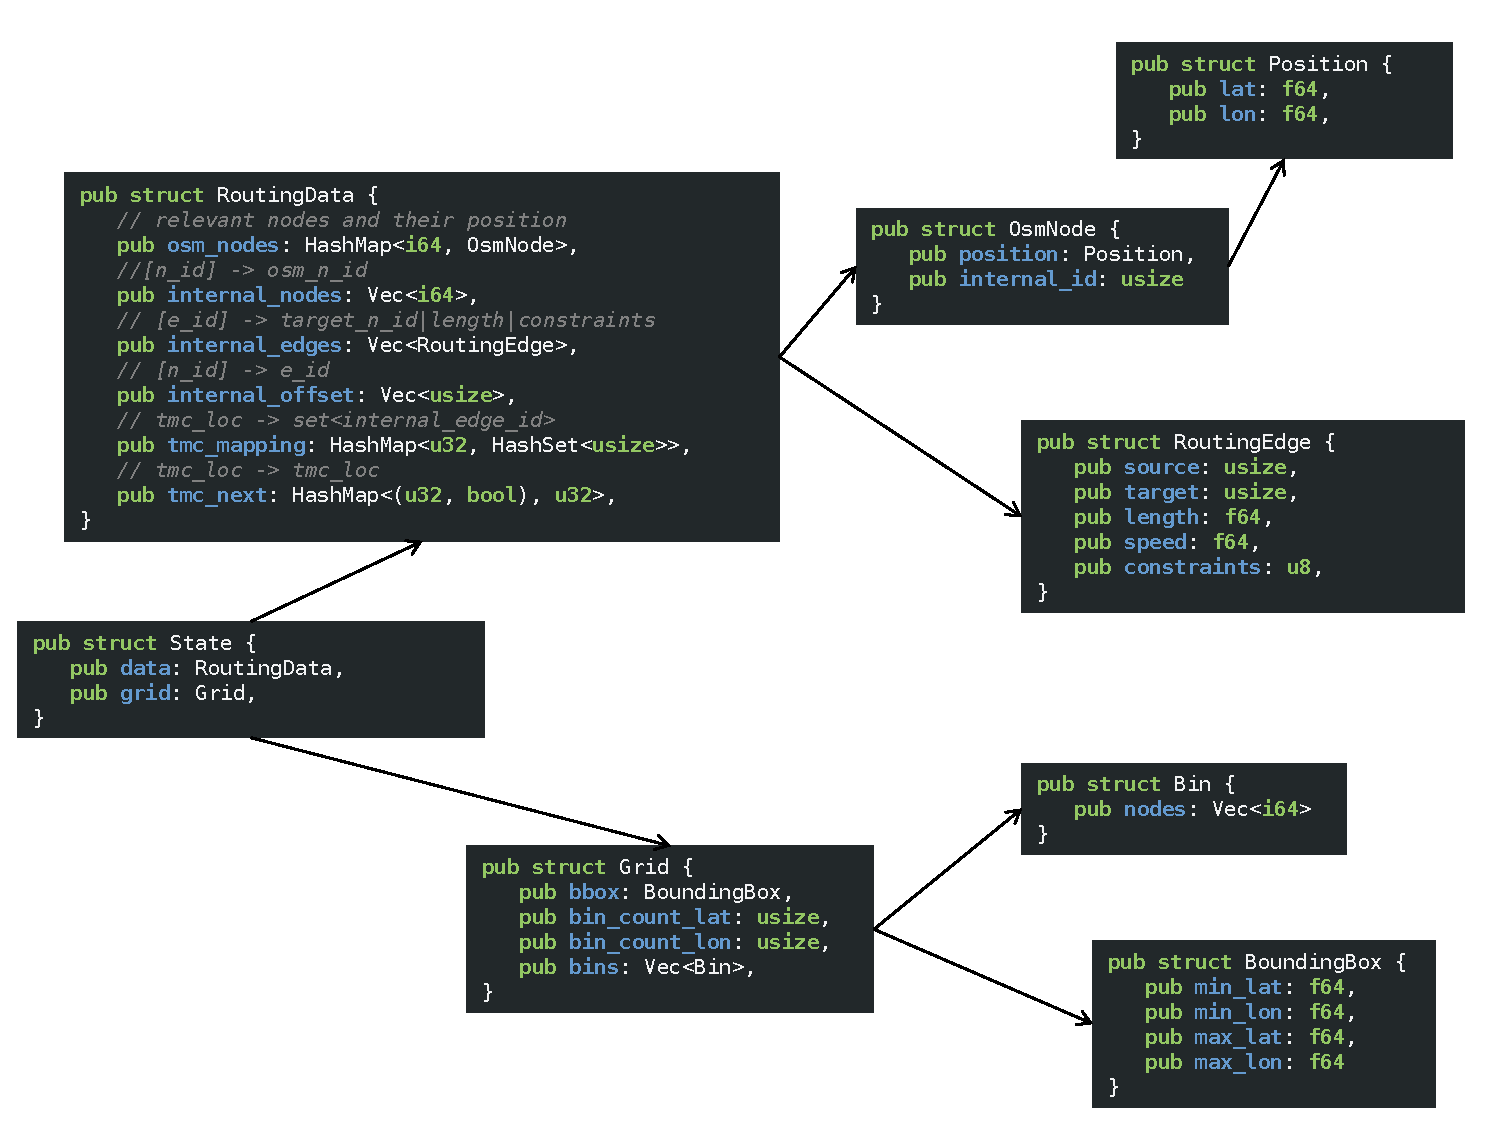
\includegraphics[width=1.0\textwidth,page=1]{img/data_structures.pdf}
\caption{Internal data representation of the routing graph.}
\label{data_routing}
\end{figure}

\subsection{Route calculation}
The shortest path is calculated using the Dijkstra algorithm. The binary heap implementation of the rust standard library is used as the data structure to keep known nodes. Depending on the vehicle (car, bike, pedestrian) edges that don't allow the chosen vehicle are skipped and depending on the metric (distance, time) and if tmc should be respected, a different cost function will be used for the edge.

\subsection{TMC handling}
\label{sec:tmc_handling}
\begin{figure}[t]
\centering
\includegraphics[width=1.0\textwidth,page=2]{img/data_structures.pdf}
\caption{Internal data representation of TMC events.}
\label{data_tmc}
\end{figure}

TMC is handled at two different points in the system. First the parser will extract two static maps containing information that is needed to handle TMC messages during runtime.
The first is a map from TMC-Location ID to a set of edge-ids and the second a map from a tuple of TMC-Location ID and boolean to TMC-Location ID. The first map is used to find the edges which are part of a location id and the second map is used to find neigboring locations of a given location and direction. While this information could also be extracted from the LCL, The new tagging scheme of OSM allows to extract this information from OSM. This has the advantage that only relevant entries are stored. 

The second point is the TMC module. This module will handle incoming TMC messages, use the second map to find all relevant location IDs and then use the first map to find the affected edges. It will then update the two maps in the TMCState struct (see Figure \ref{data_tmc}). To determine the delay of a event id, a lookup table similar to the one used in \cite{sanwald2013} was build by reading the ECL (see Table \ref{tbl:slowdown}). 
This table is translated into an if/if else/else structure for the same reasons to those given in \cite{sanwald2013}. Fields marked with * contain omitted synonyms.

\begin{table}
\centering
\begin{tabular}{ll}
\toprule
event description contains & resulting slowdown \\ 
\midrule
bridge closed* & 1.00\\ 
tunnel closed* & 1.00\\ 
stationary traffic & 0.95\\ 
queuing traffic & 0.80\\ 
slow traffic & 0.50\\ 
heavy traffic & 0.30\\ 
construction work* & 0.60\\ 
traffic problem & 0.10\\ 
accident & 0.75\\ 
\bottomrule
\end{tabular}
\caption{Lookup table used to determine the slowdown factor of an event id}
\label{tbl:slowdown}
\end{table}

Further, an extra thread will increase a counter on each entry and, if not reset by a incoming message, remove any event after 10 minutes. 

To receive TMC messages, a radio receiver is needed and from the radio signal the RDS stream has to be extracted, from which the TMC messages can then be extracted. As receiver the InstantFM Music from ADS Tech was used. The Linux Kernel contains drivers for this device. To parse the RDS stream from the radio stream, RDSD (Radio Data System daemon) was used in combination with rdsquery. RDSD and rdsquery were developed by Hans J. Koch, but the project homepage (\texttt{rdsd.berlios.de}) given in the sources is no longer available. To make RDSD and rdsquery compile on x64 ubuntu 16.04, a new include has to be added to all source files: 

\begin{verbatim}
#include <unistd.h>
\end{verbatim}
  
Running rdsd is straightforward, for rdsquery the following parameters have been used: 

\begin{verbatim}
rdsquery -s localhost -c 0 -t tmc
\end{verbatim}

This causes rdsquery to only print tmc messages to STDOUT. These have the format 
\begin{verbatim}
S evt=63 loc=12000 ext=3 dur=0 dir=1 div=0
\end{verbatim}
which is parsed by the TMC module that spawns both RDSD and RDSQUERY as child processes.


\subsection{User interface}
The UI is depicted in Figure \ref{gui}. The user can click on the map to define the source and target location and select parameters like vehicle, metric and if tmc events should be considered during routing. A route is presented as polyline on the map and the length and travel duration is listed on the sidebar on the right. TMC events are shown as red polylines with a marker and popup containing the event description and also be listed 
on the right. 

The UI is realised in JavaScript and uses leaflet to render the map and jquery to ease the communication with the API endpoints of the HTTP-Server module. 

\begin{figure}[t]
\centering
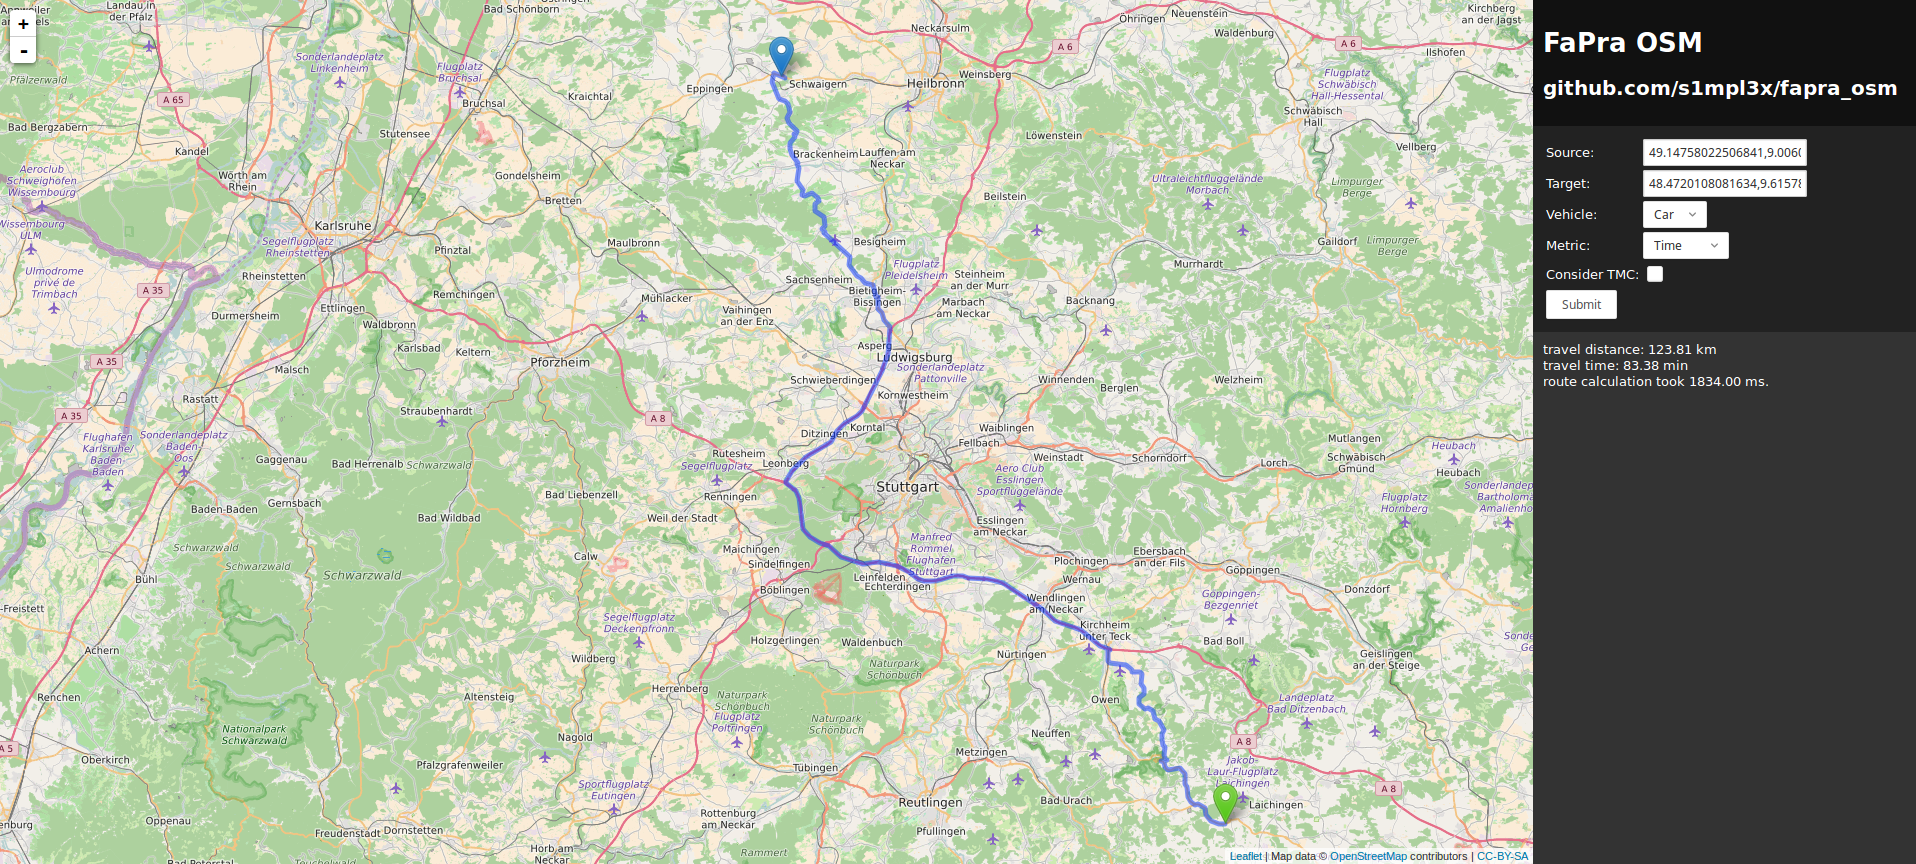
\includegraphics[width=1.0\textwidth]{img/screenshot.png}
\caption{Web-based graphical user interface}
\label{gui}
\end{figure}


\section{Implementation}
\label{impl}
The system is implemented in about 2753 lines of Rust code and about 200 lines of HTML, CSS and JavaScript for the UI\footnote{counted with CLOC \cite{cloc}}. Parsing the Baden-Würrtemberg osm.pbf file (about 400MB) takes about 3 minutes, a route calculation for this dataset typically under 2 seconds. 

\subsection{Comparision with \citetitle{sanwald2013}}
As already mentioned the systems differ in their implementation language. \citeauthor{sanwald2013} Is also using the old TMC tagging scheme. The systems also differ in the way the TMC events are handled. While sanwald directly modified the routing graph, This system keeps the TMC information separate from the graph while minimizing overhead during route calculation. Also \citeauthor{sanwald2013} uses a node delay that is applied to all incoming edges while this system directly maps the delays to the edges. While \citeauthor{sanwald2013} specifies delays in seconds, this system specifies delays as percent of the allowed max speed. The systems also differ in their data formats. While \citeauthor{sanwald2013} uses a textual representation, this system uses a binary format.

\subsection{Used third party libraries/software}
Several open source libraries were used to build this system:

\subsubsection{Rust libraries}
\begin{description}
\item[Iron]\cite{iron} HTTP-Framework for Rust.
\item[Iron-staticfile]\cite{iron_staticfile} Iron component to serve static content.
\item[Iron-mount]\cite{iron_mount} Iron middleware to map different URL-paths to different endpoints/static content.
\item[osmpbfreader-rs]\cite{osmpbfreader} Wrapper/Reader library around the pdb file format for Rust.
\item[rustc-serialize]\cite{rustc-serialize} Enables the compiler to generate serialization code to JSON/Binary representations of structs.
\item[flate2]\cite{flate2} Compression algorithms, used for compression/decompression of the state file.
\item[bincode]\cite{bincode} Used to read/write the State struct from/to disk.
\end{description}

\subsubsection{JavaScript libraries}
\begin{description}
\item[leaflet]\cite{leaflet} JavaScript map library.
\item[jquery] \cite{jquery} General helper functions.
\end{description}

\subsection{License and source code}
The source code of the presented application is available at \cite{github} and is licensed under the MIT-License:


\VerbatimInput{../LICENSE.}

\section{Conclusion and future work}
\label{concl}
In this report an application was presented that provides traffic-dependent routing. OpenStreetMap data is used as the base for the routing graph and TMC messages are used as source of current traffic information. While the application works reliably, there are several areas where improvement is possible: The parsing could be sped up by using concurrency, The coverage of TMC events could be improved and cache locality could be increased by storing nodes and edges of the graph in the built grid. 

A major limiting factor is the sparse coverage of TMC tags in the OSM data. Out of 1457361 ways in the Baden-Württemberg extract, only 2666 contained a TMC tag. In the OSM Wiki it is stated that 2906 of 3226 TMC Objects in Baden-Württemberg are tagged \cite{osm_wiki_tmc}, however it is unclear how dated that information is. Due to this fact, the majority of received TMC messages are ignored as they can't be mapped to edges in the routing graph. 

The Rust programming language proved to be suited for building this application, only the compile times and limited tooling support are minor negative points.

Possible future work includes to improve the UI with more details about TMC events and the found route, display a list of driving directions similar to popular routing applications. Other possibilities include to change the routing algorithm or to improve the memory efficiency during parsing. 

%----------------------------------------------------------------------------------------
\printbibliography
%----------------------------------------------------------------------------------------
\end{document}
